\section{Wireframes}
Let's now look at how our solution will look to the user.
\todo[inline]{add figure numbers}
Figure x contains a mockup of the guest profile editor application.
The user selects what allergens they want to avoid in their food.
Then they can choose from some of the most popular diets which they follow.
After that they can specify what food ingredients they like and dislike by writing their name to the corresponding input field and clicking the "Add" button.
When the user is finished with creating their profile, they click the "Save" button at the bottom of the screen to save their profile.

\begin{figure}[h]
  \centering
  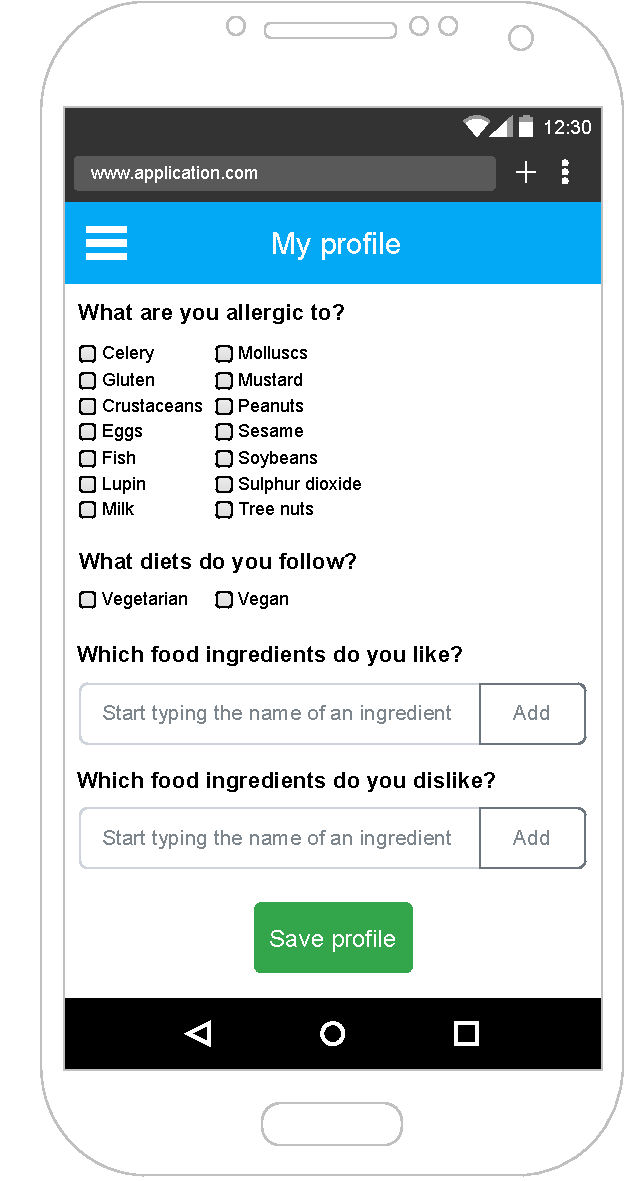
\includegraphics[width=0.62\linewidth]{master-thesis/img/wireframes/dietary_profile_editor.pdf}
  \caption{The guest profile editor application}
\end{figure}

Figure x shows what will the restaurant see when they log in to the restaurant menu maker application.


\begin{figure}[h]
  \centering
  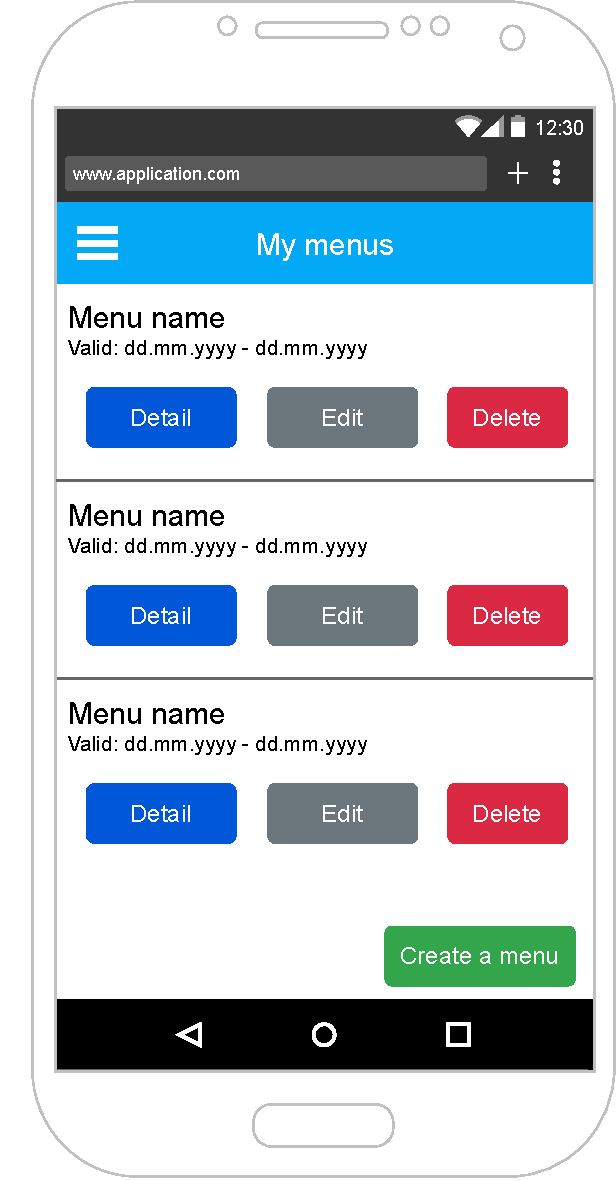
\includegraphics[width=0.62\linewidth]{master-thesis/img/wireframes/menu_creator_menus_overview.pdf}
  \caption{The restaurant menu maker application}
\end{figure}

\begin{figure}[h]
  \centering
  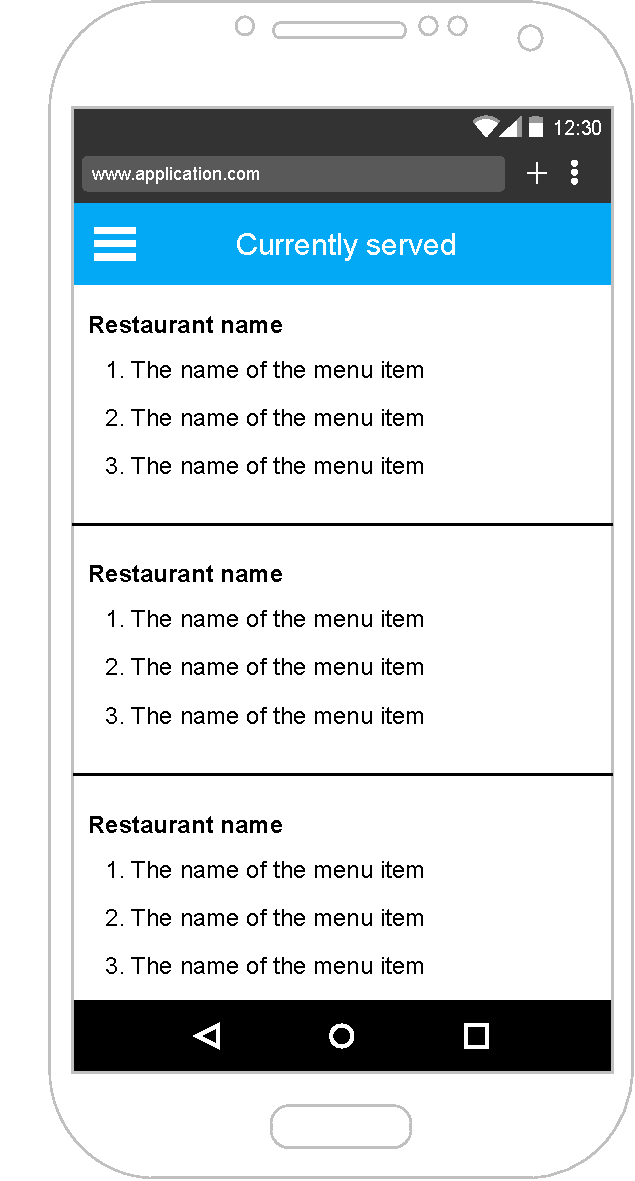
\includegraphics[width=0.62\linewidth]{master-thesis/img/wireframes/menu-viewer-currently-served.pdf}
  \caption{The personalized menu viewer application's home page}
\end{figure}

\begin{figure}[h]
  \centering
  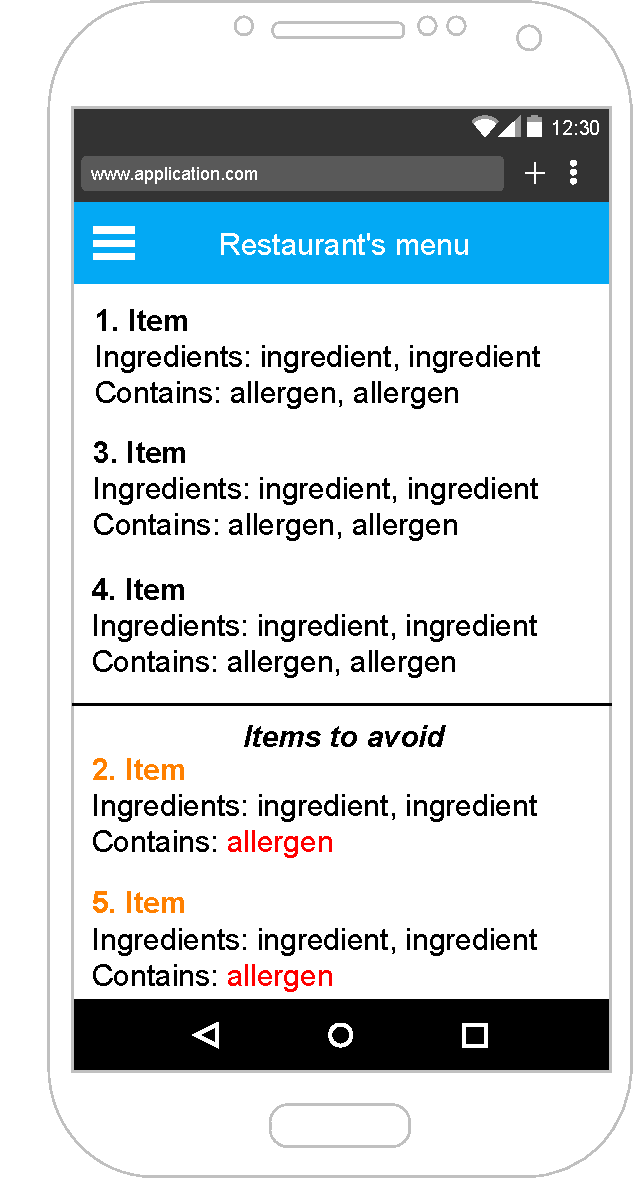
\includegraphics[width=0.62\linewidth]{master-thesis/img/wireframes/menu_viewer_menu_detail.pdf}
  \caption{The personalized menu viewer application's menu detail}
\end{figure}
